\ca{\chapter{Implementation}}
\renewcommand{\baselinestretch}{\mystretch}
\label{chap:Impl}
%\setlength{\parindent}{0pt}

\PARstart{\ca{S}}{\ca{everal}} \ca{%
implementations of various portions of the final optimised controller application were developed independently, so that each portion can be verified working before integration. The implementations were developed as the following steps:
}

\begin{enumerate}[noitemsep,leftmargin=4cm]
  \item[Qt2 demo:] A controller specific application using C++ with Qt2-based GUI, to test the performance of the NP1380 platform and showcase an interactive application design.
  \item[\texttt{VixenLinky}:] C\# implementation of a controller specific application, for use as the references of the optimal performances on different platforms.
  \item[Playback engine:] Integrate the sequence decoding routine from \texttt{VixenLinky} to the Vixen application as a separate playback engine.
  \item[\texttt{VixenConsole}:] A command-line interface (CUI) version of the Vixen application, but with only minimal functionalities and a working playback engine for embedded platforms.
  \item[Video transcoding:] Various programs for video processing, integrated into the playback engine for video format support.
\end{enumerate}

\clearpage

\section{\ca{Qt2-based} implementation}

A GUI application dedicated to the \texttt{TCPLinky} controller was developed using C++ as \ca{a user-friendly alternative implementation} showcase. This application was developed specific to the Noah NP1380 platform listed in \sref{sec:systems}. This device is a handheld embedded device based on a 10 years old SoC chip, originally designed for educational use \ca{such as electronic dictionaries}. Fortunately, this devices uses Linux system and Qt2 as GUI. Therefore, it is possible to test Vixen application on this low-end platform.

\begin{figure}[t]
  \centering
  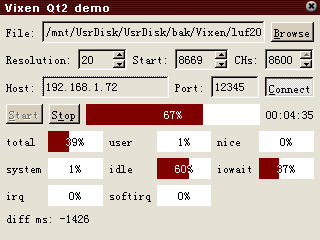
\includegraphics[width=0.45\textwidth]{Figs/vixen_noah.png}%
  \caption{\footnotesize Screenshot of Vixen Qt2 demo on Noah NP1380}
  \label{fig:vixen_noah}
\end{figure}

\fref{fig:vixen_noah} shows a screenshot of the dedicated application. The method of performance profiling through statistic files in proc file system was also tested. These smaller progress bars at the lower half of the application shows percentages of CPU time spent on different tasks, such as user space applications, kernel mode and interrupt handling. Most of the time only less than $50 \%$ CPU time was used for this controller application, \ca{indicating that} even this low-end device is capable of handling thousands of lighting channels.

\section{Minimal C\# implementation}

To set up a reference baseline for optimal performance \ca{of the new playback engine}, sequence rendering application \ca{named \texttt{VixenLinky} was developed.}

\ca{\subsection{Implementation}}

\ca{\texttt{VixenLinky} was implemented using C\#, takes} the same \ca{``Raw''} sequence data \ca{format}, but \ca{supports} only the \texttt{TCPLinky} controller developed in \sref{sec:tcplinky}. \ca{It was} implemented as \ca{simply} as possible without all intermediate layers \ca{and module loading routines}, but still \ca{using} a threading structure \ca{identical to} the original Vixen application. \ca{The source code for controlling the \texttt{TCPLinky} controller} was ported directly from the original Vixen application \ca{to ensure compatibility and similarity}.

\ca{\subsection{Purpose}}

With this program, the \ca{ideal} performance \ca{of the new playback engine} on each platform can be measured. The \ca{remaining performance limitation factors are} sequence loading performance and controller update speed. Therefore, options to unlimit the update interval of both sequence loading and controller update were added separately \ca{for the measurements of maximum update rates}.

\fref{fig:vixenlinky_noah} shows an example of performance data gathered on the Noah NP1380 platform through \texttt{VixenLinky} using \ca{the exported test sequence}. The refresh rates of both playback and controller \ca{were} very stable around \ca{the configured} 50 fps. The CPU usage \ca{peaked} at $60.0 \%$\ca{,} while most of the time it \ca{was} distributed around $20.0 \%$ and $30.0 \%$ (first and third quartiles).

\begin{figure}[!t]
  \centering
  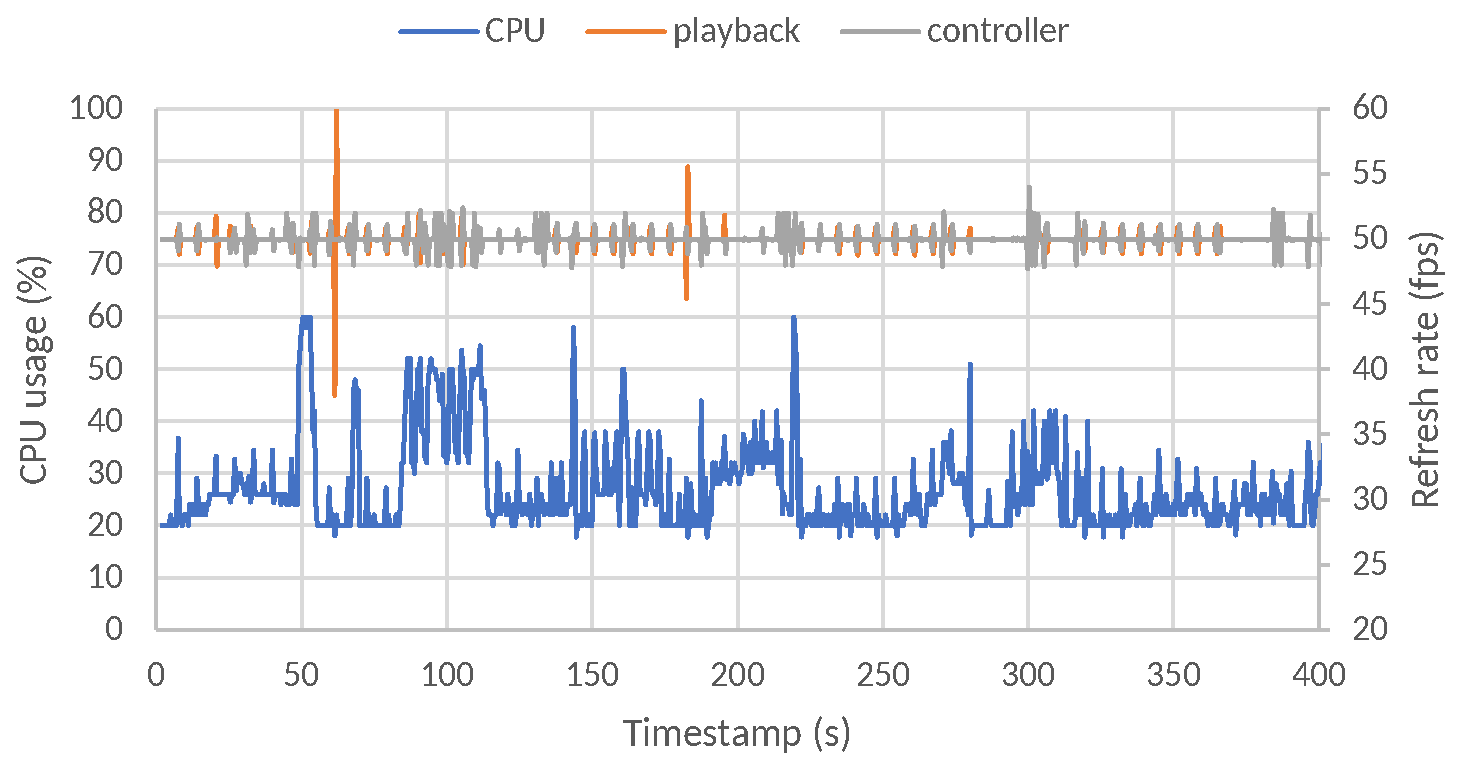
\includegraphics[width=0.8\columnwidth]{Figs/vixenlinky_noah.eps}
  \caption{\footnotesize Performance of \texttt{VixenLinky} on Noah NP1380}
  \label{fig:vixenlinky_noah}
\end{figure}

\section{Playback engine}

After \ca{verifying} the ability \ca{to load and render} the exported lighting \ca{sequences} by controller specific \ca{applications}, the C\# code for loading exported sequence \ca{from \texttt{VixenLinky}} was integrated into Vixen application as a separate playback engine.

\subsection{Implementation}

The playback engine starts by reading the exported network XML file. To simplify the process, \ca{an} XML object serialiser was used to interpret \ca{and store} the XML \ca{data structure} to a similarly structured C\# object for later access. The information \ca{read} from XML will be used to determine controller channel mapping, update interval and optional audio media file. To further reduce \ca{matching} overhead, the controller names will be looked up and converted to their unique ID (GUID) \ca{instead}. The optional audio media file was supported by utilising the same audio media functions from original execution engine.

All preview, element and filter updates were skipped in the playback engine. The translation layers were skipped, since the sequence data is already specific to the controllers. However, in order to match the existing interface of controller modules, \ca{segments of sequence data frame buffer} still need to be copied again \ca{as command batches for each controllers}, incurring some unnecessary overhead.

The structure of update management was also changed\ca{, as illustrated in \fref{fig:update}}. \ca{In the original execution engine}, the application updates \ca{data buffers} from \ca{controller update requests}, which requires the use of mutex \ca{locks to coordinate} data \ca{accesses} between controller threads. With a configuration \ca{consists} of multiple controllers, potential lock contention of the mutex can also incur some overhead. \ca{To address this issue, another} thread dedicated to sequence loading was \ca{added} to the playback engine, similar to the structure of controller specific implementations. In this way, only the sequence loading thread may update the channel data buffer, \ca{removing} the need of mutex \ca{locks}.

\begin{figure*}[t]
  \centering
  \subfloat[Execution engine]{\frame{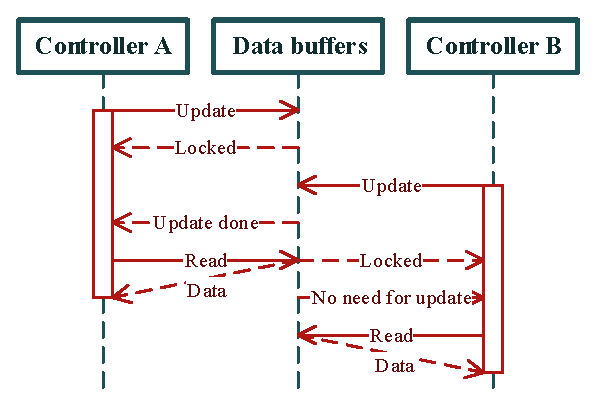
\includegraphics[height=4cm]{Figs/update_execution.eps}}}
  \hfil
  \subfloat[Playback engine]{\frame{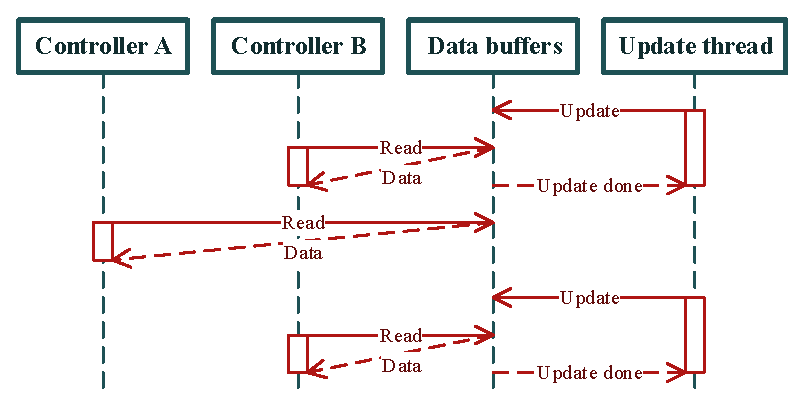
\includegraphics[height=4cm]{Figs/update_playback.eps}}}
  \caption{\footnotesize Update management of Vixen engines}
  \label{fig:update}
\end{figure*}

One major drawback of using the playback engine is that the \ca{exported} data cannot be mapped back to element states yet\ca{, which is essentially the reverse of export}. Therefore, editing the \ca{exported} sequence using the built-in editor and the preview output were not supported.

\subsection{Integration}

Several code branches were added to switch between the original execution engine and the new playback engine. The execution engine was still used as the default engine to simplify status checking and support the sequence editor. The playback engine will be switched to \ca{only if an exported sequence was loaded to it and started rendering}.

A simple control dialog was added as a menu entry for the \ca{new playback} engine, as shown \ca{in} \fref{fig:vixen_playback}. More complex and user-friendly UI design is possible, however, due to limited time \ca{constraints} this control dialog should be sufficient for this project and proof of concept.

\begin{figure}[t]
  \centering
  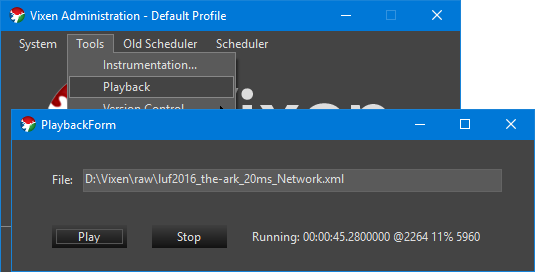
\includegraphics[width=0.8\columnwidth]{Figs/vixen_playback.png}
  \caption{\footnotesize Screenshot of the playback engine control dialog}
  \label{fig:vixen_playback}
\end{figure}

The playback control was also integrated \ca{as a new type of action into the} built-in schedulers. It can therefore be scheduled to execute at specific \ca{times with different sequences}, possibly \ca{together with other existing actions including} schedules using the original execution engine. The new playback engine does not need additional pre-process for show schedules, \ca{and} can be directly started within seconds.

\section{Console application}

\ca{To improve the usability of the new playback engine on Linux-based platforms especially embedded platforms, a} Command-line User Interface (CUI) version of Vixen, named \texttt{VixenConsole}, was implemented. It is easier to operate and manage a CUI based program through remote connection \ca{and automated scripts} instead of a distorted partially functional GUI application \ca{on Linux}. \cref{chap:Guide} \ca{lists} the detailed usage description of \texttt{VixenConsole}.

\ca{Different from the reference implementation \texttt{VixenLinky} that only supports the \texttt{TCPLinky} controller, this \texttt{VixenConsole} application is a simplified version of the Vixen GUI application, supports all controller modules the Vixen GUI application supports.}

\ca{\subsection{Implementation}}

The original core codebase from \texttt{Vixen.dll} was used in this program with some necessary modifications. Instead of full initialisation from Vixen GUI application, only \ca{available controllers modules and their configurations} will be \ca{loaded during start-up by} \texttt{VixenConsole} to reduce overheads. In this way, the code for the playback engine, module and data loading is \cad{still} shared with the Vixen GUI application, \ca{can also receive} future improvements and patches.

\texttt{VixenConsole} reads configurations from the same location as Vixen application, the \texttt{Vixen 3} folder from user home directory. All configurations are stored as XML files, exported directly from settings object using XML serialiser. The ability to list available controllers and their configurations \ca{was} added to \texttt{VixenConsole}. However, configuration modification was not yet possible from \texttt{VixenConsole}, due to the complexity of supporting every \ca{possible} types of configuration fields within the project time constraint. To create or modify the configuration, the Vixen GUI application can be used from a computer running Microsoft Windows. Editing the XML configuration files directly using text editors is also possible.

\ca{\subsection{Scheduling}}

\ca{
The \texttt{VixenConsole} application does not have a build-in show scheduler. Instead, existing job scheduler utilities such as \texttt{crontab} \cite{crontab} can be used, since the \texttt{VixenConsole} application with the new playback engine does not have a pre-rendering step, therefore can be started within a reasonable amount of time. Together with the help of Linux shell scripting, this way of scheduling can be much more flexible than a fixed time scheduler. To reduce start-up time, back-to-back playback of multiple sequences were also supported.
}

\section{Video data format}

With the implementation of \texttt{VixenConsole}, the process of designing and pre-rendering (exporting) the sequence on Vixen application then playback later using \texttt{VixenConsole} became very similar to the process of video editing and playback. Therefore, it \ca{was thought to} be beneficial to add support for video sequence format.

\subsection{Implementation}

The open source \texttt{ffmpeg} framework \cite{ffmpeg} was used for video processing. The open source nature ensures up-to-date version of \texttt{ffmpeg} is available on all testing platforms.

The \texttt{ffmpeg} framework uses the C programming language for its API. The complicity of different data structures used by \texttt{ffmpeg} results in no up-to-date C\# wrapper API available for use directly. Therefore, an intermediate wrapper layer between Vixen and \texttt{ffmpeg} was developed to encapsulate all complex \texttt{ffmpeg} routines using C.

The development of video integration was separated into multiple steps. Firstly, several C programs were developed to test individual video processing functions including video encoding, video decoding, stream muxing and metadata \ca{retrieval}. Afterwards, working code segments were combined into a dynamic library, with a simplified API suitable for C\#. A C\# wrapper class was then developed using the \texttt{InterOp} service \cite{interop}, together with another C\# program for testing video encoding and decoding. After all these small testing programs had been confirmed working, the C\# wrapper was finally integrated into Vixen with the playback engine. The playback engine checks for \ca{the} input file extension to determine whether to load the file as \ca{an} exported ``Raw'' sequence or \ca{a} video file.

\ca{The default video encoding format for encoding exported sequences is \texttt{h264} with \texttt{rgb24} pixel format.} It is possible to add support for multiple video formats as options to the \ca{wrapper} library to directly transcode from ``Raw'' sequence to other video formats. However, this can make the encoding process \ca{and export options} over complicated. Instead, other dedicated video transcoding tools can be used for the same task. The decoding routine used in playback engine was designed to support any video encoding format, by converting the video frames to \texttt{rgb24} format internally.

To ensure lossless transcoding from the ``Raw'' sequence to \ca{a} video stream, the transcoding programs were tested by encoding example sequences to \ca{videos} then decoded back to \ca{new sequences}. The \ca{new} sequences were then compared for any difference \ca{to the original sequence}, using the GNU \texttt{diff} tool \cite{diff}. Makefile was used for automated \ca{compilation} and testing.

To minimise number of files needed for playback, the optional audio file was muxed together with the video stream, and the network configuration XML file was stored directly as \ca{a} string literal in \ca{a} video metadata field \ca{named} ``comment'', as shown \ca{in} \fref{fig:video-info}.

\begin{figure}[t]
  \centering
  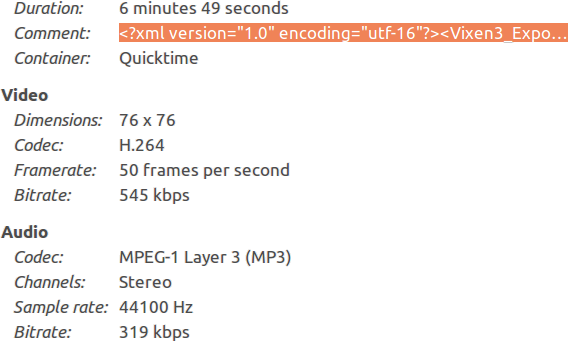
\includegraphics[width=0.7\textwidth]{Figs/video_info.png}
  \caption{\footnotesize Media information of an example video sequence}
  \label{fig:video-info}
\end{figure}

\subsection{Rendering}

In the playback engine, video frames will be transformed to controller data frames for rendering. However, the existing audio rendering engine \texttt{FMOD} from Vixen only supports media file playback. The required functionality of playing decoded \ca{audio} data frames was not available from its C\# API. To resolve this issue, C code for operating a newer version of \texttt{FMOD} was added to the wrapper library. The playback engine transfers the decoded audio frame back to the wrapper library for audio playback.

\cmt{Therefore, audio playback using the ``Raw'' sequence was unsupported by \texttt{VixenConsole}.}

It is possible to support audio playback with exported ``Raw'' sequences using the newer version of \texttt{FMOD}. However, this was not implemented yet.

\cmt{TODO: Implement audio playback with ``Raw'' sequence, update performance data}
